\section{Visual Servoing Simulation Results}
The proposed visual servoing control scheme was validated in a simulation environment to assess its baseline behavior. The results presented in Figure~\ref{fig:sim_results} were obtained using uncalibrated controller parameters (i.e., nominal gains without specific tuning).

Figure~\ref{fig:sim_results}a illustrates the 3D Cartesian trajectory of the camera end-effector. Despite the use of uncalibrated parameters, the system successfully generates a smooth path from the starting pose (green marker) to the desired end pose (red marker).



The corresponding image-space behavior is shown in Figure~\ref{fig:sim_results}b, where the four feature points traverse from their initial detections (circles) to the desired target locations (stars). The curvature observed in these trajectories is characteristic of the Image-Based Visual Servoing (IBVS) control law, which decouples the 2D image error correction from the 3D Cartesian path.


\begin{figure}[H]
    \centering
    % Figure A
    \begin{subfigure}[b]{0.48\textwidth}
        \centering
        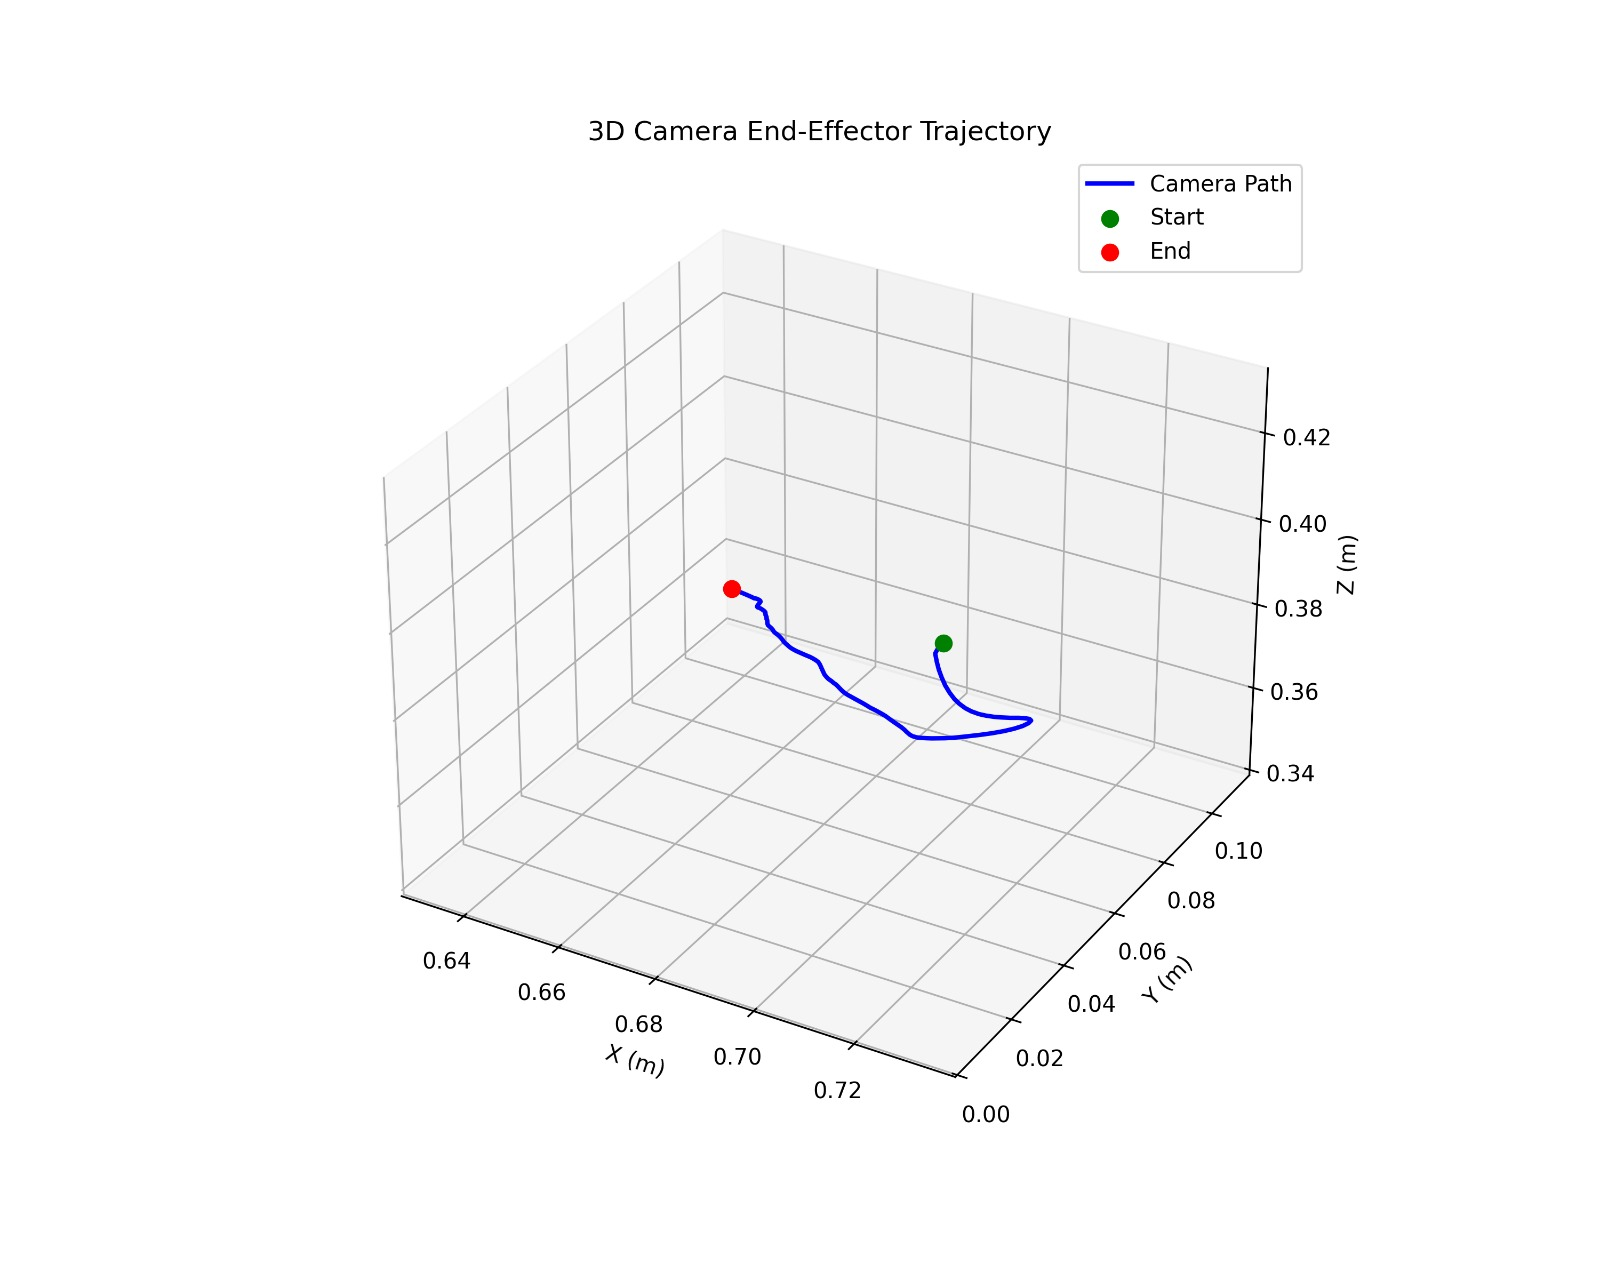
\includegraphics[width=\textwidth]{Figures/chapter4/Visual Servo/thesis_cartesian_path.jpeg}
        \caption{3D Camera End-Effector Trajectory}
        \label{fig:cartesian_path}
    \end{subfigure}
    \hfill
    % Figure B
    \begin{subfigure}[b]{0.48\textwidth}
        \centering
        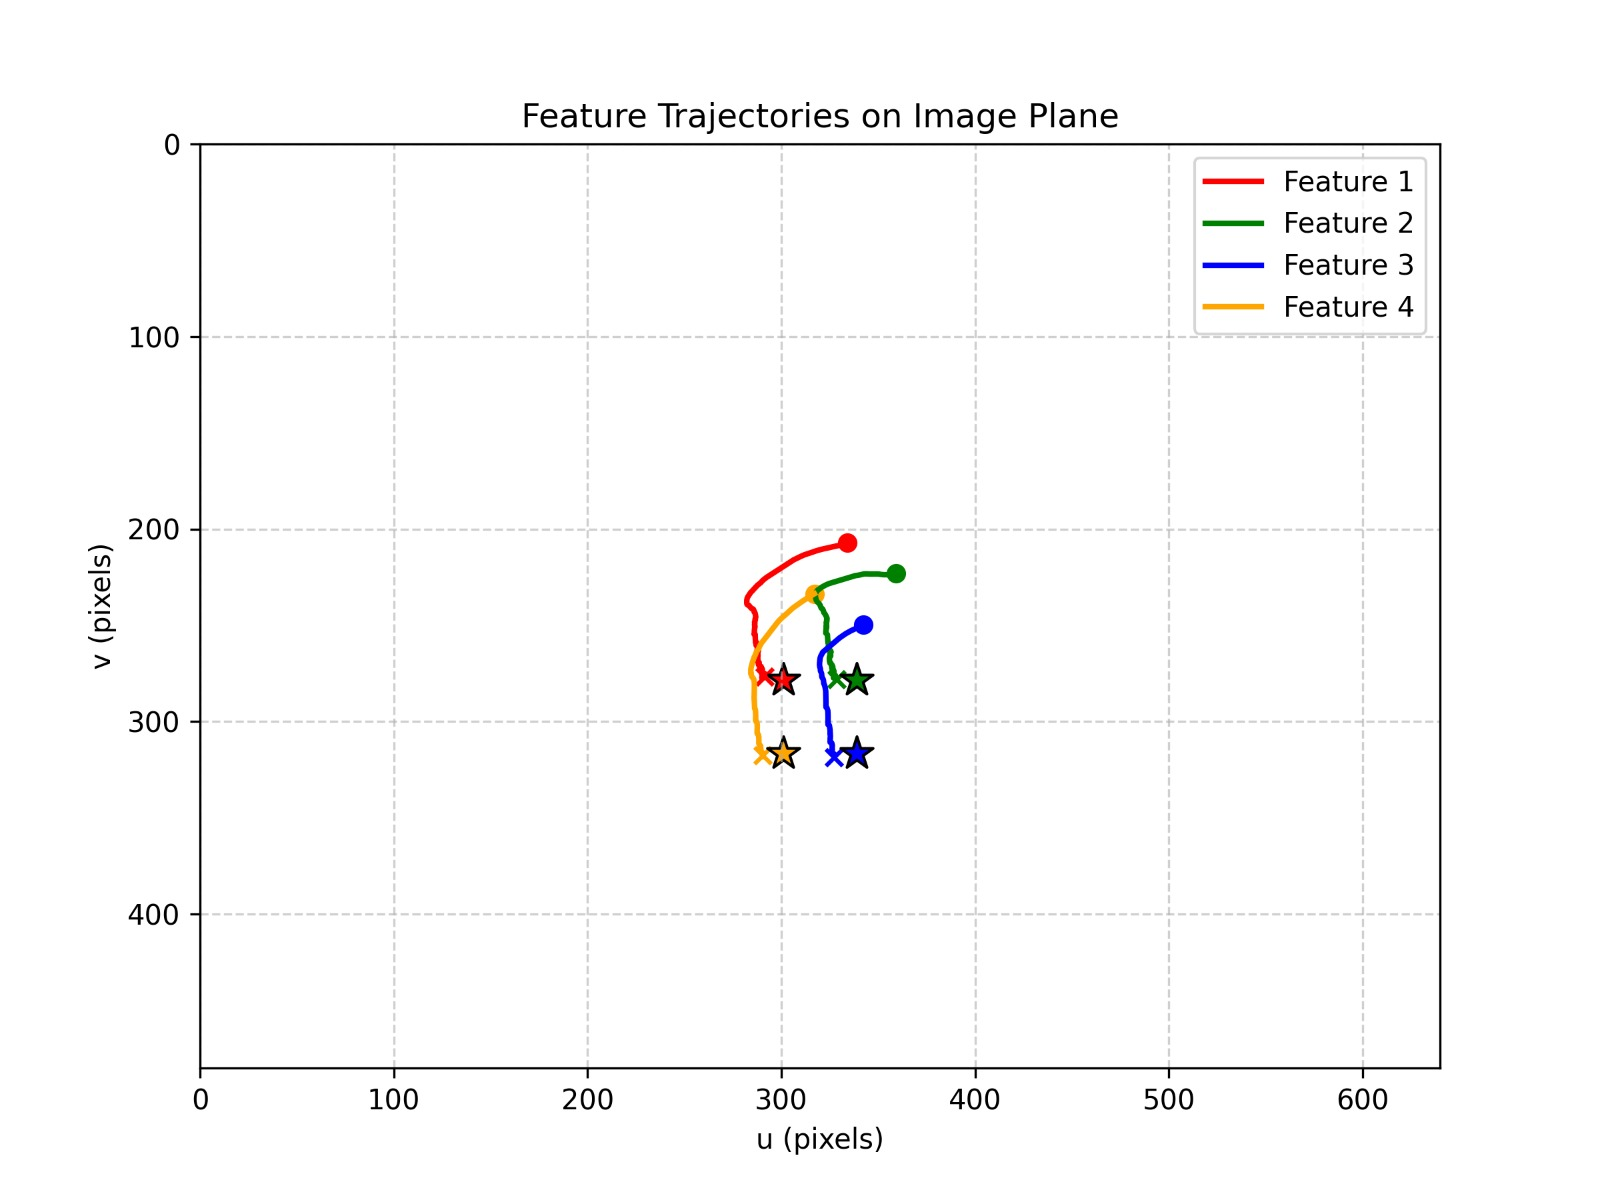
\includegraphics[width=\textwidth]{Figures/chapter4/Visual Servo/thesis_image_trajectory.jpeg}
        \caption{Feature Trajectories on Image Plane}
        \label{fig:image_traj}
    \end{subfigure}
    
    \vspace{0.5cm}
    
    % Figure C
    \begin{subfigure}[b]{0.7\textwidth}
        \centering
        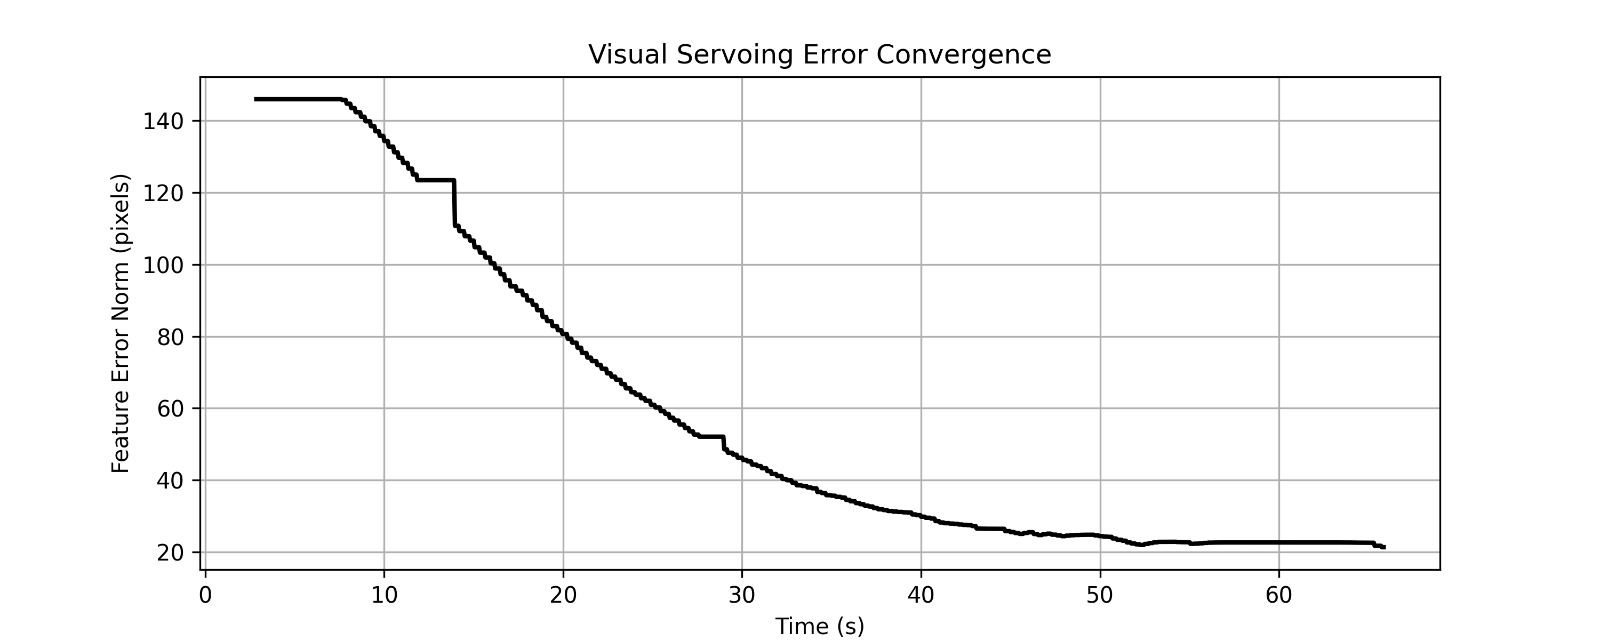
\includegraphics[width=\textwidth]{Figures/chapter4/Visual Servo/thesis_error_convergence.jpeg}
        \caption{Visual Servoing Error Convergence}
        \label{fig:error_conv}
    \end{subfigure}
    
    \caption{\textbf{Simulation Results (Uncalibrated Parameters):} Performance of the IBVS controller in a simulation environment using uncalibrated controller parameters. (a) The Cartesian path of the camera frame. (b) The trajectories of the four feature points in the image plane ($u, v$) converging to the desired targets (stars). (c) The monotonic decrease of the error norm, demonstrating convergence despite the lack of parameter tuning.}
    \label{fig:sim_results}
\end{figure}
Finally, Figure~\ref{fig:sim_results}c confirms the stability of the system. The feature error norm decreases monotonically over time, converging to zero without significant oscillation. This demonstrates that the control law remains effective and ensures convergence even when operating with uncalibrated controller parameters.